\documentclass[conference]{IEEEtran}
\IEEEoverridecommandlockouts

\usepackage[utf8]{inputenc}
\usepackage[T1]{fontenc}
\usepackage{amsmath,amssymb}
\usepackage{graphicx}
\usepackage{booktabs}
\usepackage{multirow}
\usepackage{siunitx}
\usepackage{xcolor}
\usepackage{url}
\usepackage[hidelinks]{hyperref}
\usepackage{cite}
\usepackage[section]{placeins}
\renewcommand{\topfraction}{0.9}
\renewcommand{\bottomfraction}{0.8}
\renewcommand{\textfraction}{0.07}
\renewcommand{\floatpagefraction}{0.75}
\renewcommand{\dbltopfraction}{0.9}
\renewcommand{\dblfloatpagefraction}{0.75}
\setcounter{topnumber}{3}
\setcounter{bottomnumber}{2}
\setcounter{totalnumber}{6}
\setcounter{dbltopnumber}{2}

\graphicspath{{figures/}}
\sisetup{group-separator={,}, group-minimum-digits=4}

\begin{document}

\title{Benchmarking Classical Machine Learning for Four-Level Depression Severity Classification from Text: A Leakage-Controlled Comparison of Bag-of-Words and TF-IDF Representations}

\author{\IEEEauthorblockN{Raghav Vashisht, Aanandit Kanwar, Apurav Gautam}
\IEEEauthorblockA{Department of Computer Science and Engineering\\
Chitkara Institute of Engineering (CUIET)}}

\maketitle

% ---------------------------------------------------------------------------
\begin{abstract}
Depression is a leading cause of disability worldwide, yet it remains under-diagnosed because of stigma, self-report bias and limited access to clinicians. Automated analysis of user-written text offers a scalable, non-invasive route to early screening. This paper benchmarks three classical machine-learning classifiers---Naive Bayes, Logistic Regression and Random Forest---paired with two lexical feature representations, Bag-of-Words (BoW) and Term Frequency--Inverse Document Frequency (TF-IDF), for four-level depression severity classification (Minimal, Mild, Moderate, Severe) on the publicly available Depression Severity Levels Dataset (\num{41873} posts). A data audit performed before modelling found that 29.9\% of the rows were exact duplicates or texts carrying contradictory severity labels, and that the apparent class balance of the corpus was produced largely by duplicating Moderate posts. After de-duplication, \num{29328} unique posts remained and the Moderate class shrank by 81.6\%. On this leakage-controlled corpus, Logistic Regression with TF-IDF features achieved the highest macro-averaged F1-score of 0.661 (accuracy 0.691), and the best recall on the clinically critical Severe class was 0.703 (Naive Bayes, BoW). L1-regularised Logistic Regression attributed Severe predictions mainly to explicit suicidal-ideation terms together with the first-person pronoun ``I'' and the negation ``cannot'', words that standard stop-word lists remove. Evaluating on the corpus as distributed shifted macro-F1 by $-1.5$ to $+3.7$ points, because duplicated posts inflate and contradictorily labelled posts deflate scores, so results computed on the raw file are not comparable in either direction. Classical models trained in seconds to minutes on commodity hardware and remain transparent, supporting their use as auditable first-stage screening aids ahead of formal clinical evaluation.
\end{abstract}

\begin{IEEEkeywords}
depression severity, natural language processing, TF-IDF, bag-of-words, random forest, logistic regression, naive Bayes, data leakage, mental-health screening
\end{IEEEkeywords}

% ---------------------------------------------------------------------------
\section{Introduction}

Depressive disorders affect an estimated 280 million people globally and are a leading contributor to the global burden of disability~\cite{who2023depression}. Standardised instruments such as the Beck Depression Inventory (BDI)~\cite{beck1996bdi2,beck1988psychometric} and the Patient Health Questionnaire (PHQ-9)~\cite{kroenke2001phq9} grade symptom severity, but administering them requires contact with a clinician or a deliberate act of self-assessment, which stigma and limited mental-health resources often prevent. Meanwhile, people increasingly describe their emotional state in writing---on forums, social media and support communities---producing text that carries measurable linguistic correlates of depression~\cite{rude2004language,dechoudhury2013predicting}.

Most computational work on this signal frames depression as a binary problem (depressed vs.\ not depressed)~\cite{dechoudhury2013predicting,coppersmith2014quantifying}. Clinical practice, however, is graded: a Mild presentation and a Severe one call for very different responses, and missing a Severe case is far costlier than over-flagging a Mild one. Multi-level severity datasets have recently become available~\cite{naseem2022early,sampath2022dataset}, but three gaps remain.

\begin{enumerate}
  \item \textbf{Benchmark gap.} Severity work increasingly favours deep and transformer models, while transparent classical baselines on the same four-level task are rarely reported with a full, reproducible hyper-parameter protocol.
  \item \textbf{Data-quality gap.} Severity corpora are often aggregated from several sources. Duplicate and contradictorily labelled posts can then fall on both sides of a train/test split, a form of leakage known to inflate reported performance~\cite{kapoor2023leakage,lee2022dedup}. To our knowledge this has not been quantified for depression-severity text.
  \item \textbf{Interpretability gap.} Screening tools must be auditable, yet the lexical features that push a multi-level severity classifier towards a Severe prediction are seldom reported.
\end{enumerate}

This paper makes four contributions: (i)~a pre-modelling audit of the Depression Severity Levels Dataset that identifies and removes conflicting and duplicate records; (ii)~a leakage-controlled benchmark of Naive Bayes, Logistic Regression and Random Forest under BoW and TF-IDF features, tuned by exhaustive grid search with stratified five-fold cross-validation; (iii)~a sensitivity analysis showing how evaluating on the raw corpus would have changed the results; and (iv)~an interpretability analysis of the linguistic markers most associated with Severe predictions. The complete pipeline is scripted end to end, so every number in this paper can be regenerated from the public dataset.

% ---------------------------------------------------------------------------
\section{Related Work}

\textbf{Depression detection from user text.} De~Choudhury et al.~\cite{dechoudhury2013predicting} showed that behavioural and linguistic features of social-media activity predict a later depression diagnosis, and Coppersmith et al.~\cite{coppersmith2014quantifying} quantified mental-health signals on Twitter using self-reported diagnoses. Shared tasks such as CLEF eRisk~\cite{losada2016test} and Reddit-based corpora~\cite{yates2017depression} formalised early-risk detection, again mostly as a binary or risk-ranking problem. Guntuku et al.~\cite{guntuku2017detecting} review this literature and highlight label quality and generalisability as recurring weaknesses.

\textbf{Severity-level datasets.} Naseem et al.~\cite{naseem2022early} re-annotated Reddit posts into four depression severity levels and proposed an ordinal classification approach. Sampath and Durairaj~\cite{sampath2022dataset} released a social-media dataset graded as not depressed, moderate and severe. The Depression Severity Levels Dataset used here aggregates publicly available corpora into four BDI-aligned bands~\cite{kuas2023dataset}. A domain lexicon for depression detection~\cite{cha2022lexicon} is referenced by the dataset authors and motivates our planned lexicon-augmented experiment.

\textbf{Linguistic markers.} Rude et al.~\cite{rude2004language} found that depressed students use the first-person singular pronoun ``I'' more often, and Al-Mosaiwi and Johnstone~\cite{almosaiwi2018absolute} identified absolutist words (``always'', ``nothing'', ``completely'') as a marker specific to depression, anxiety and suicidal ideation. Both findings matter for preprocessing: generic stop-word lists delete exactly these words.

\textbf{Classical vs.\ deep models.} Transformer models dominate recent leaderboards, but classical linear and ensemble models remain competitive on short, lexically rich text and are far cheaper to train, deploy and explain~\cite{guntuku2017detecting}. Complement Naive Bayes~\cite{rennie2003tackling}, L1-regularised logistic regression~\cite{tibshirani1996lasso,zou2005elasticnet} and Random Forests~\cite{breiman2001rf} are standard, well-understood baselines for this setting.

\textbf{Leakage and duplication.} Kapoor and Narayanan~\cite{kapoor2023leakage} document data leakage as a pervasive cause of over-optimistic results in ML-based science, and Lee et al.~\cite{lee2022dedup} show that de-duplicating training data materially changes model behaviour and evaluation. We apply this lens to depression-severity text.

% ---------------------------------------------------------------------------
\section{Methodology}

\subsection{Dataset and Audit}

The Depression Severity Levels Dataset~\cite{kuas2023dataset} is distributed as a single CSV with two columns, \texttt{text} and \texttt{label}. Labels follow four severity bands that the dataset authors align to BDI cut-offs: Minimal (0--9), Mild (10--18), Moderate (19--29) and Severe (30--63)~\cite{beck1988psychometric}. These labels are \emph{annotations of text} under the authors' Depression Severity Annotation Schema (DSAS); they are not questionnaire scores obtained from the authors of the posts and must not be interpreted as clinical diagnoses.

Before modelling we audited the corpus (Table~\ref{tab:audit}). Exact-duplicate texts were common, and \num{3053} unique texts appeared with more than one severity label---\num{3028} of them labelled both Minimal and Moderate, which points to a systematic mapping inconsistency between source corpora rather than random annotator disagreement. Because no correct label can be recovered for such texts, every copy of a conflicting text was removed. Remaining exact duplicates were collapsed to one instance. After text normalisation (Section~\ref{sec:prep}), 32 posts with no remaining tokens were also dropped.

\begin{table}[!htbp]
\centering
\caption{Corpus audit}
\label{tab:audit}
\begin{tabular}{lrr}
\toprule
Step & Removed & Remaining \\
\midrule
Raw corpus & -- & \num{41873} \\
Empty text & 14 & \num{41859} \\
Conflicting labels (\num{3053} texts, all copies) & \num{6305} & \num{35554} \\
Exact duplicates & \num{6194} & \num{29360} \\
Empty after preprocessing & 32 & \textbf{\num{29328}} \\
\bottomrule
\end{tabular}
\end{table}

\begin{table}[!htbp]
\centering
\caption{Class distribution before and after the audit}
\label{tab:classes}
\begin{tabular}{lrrr}
\toprule
Class & As distributed & After audit & Change \\
\midrule
Minimal  & \num{10556} & \num{6280}  & $-40.5\%$ \\
Mild     & \num{10661} & \num{10638} & $-0.2\%$ \\
Moderate & \num{9480}  & \num{1744}  & $-81.6\%$ \\
Severe   & \num{11176} & \num{10666} & $-4.6\%$ \\
\midrule
Total    & \num{41873} & \num{29328} & $-30.0\%$ \\
\bottomrule
\end{tabular}
\end{table}

Individual Moderate posts were repeated up to 14 times in the distributed file, so the near-uniform class balance reported for the corpus is largely an artefact of duplication (Table~\ref{tab:classes}). The audited corpus is imbalanced (Moderate $=5.9\%$), which we address through class weighting and macro-averaged metrics rather than resampling.

\subsection{Preprocessing}\label{sec:prep}

Each post was (1)~lower-cased with apostrophes normalised; (2)~stripped of URLs and user mentions; (3)~expanded for negative contractions (``can't''~$\to$~``can not'', ``don't''~$\to$~``do not''); (4)~stripped of non-alphabetic characters; (5)~filtered for stop words; and (6)~lemmatised with WordNet (noun, then verb form).

Stop-word removal used the scikit-learn English list~\cite{pedregosa2011sklearn} \emph{minus} depression-relevant function words: first-person pronouns (\textit{i, me, my, mine, myself, we, us, our}), negations (\textit{no, not, nor, never, none, nobody, nothing, nowhere, neither, cannot}) and the affect-bearing words \textit{alone, empty, against, without} and \textit{cry}, all of which the stock list removes. Retaining them follows the evidence on pronoun use~\cite{rude2004language} and absolutist language~\cite{almosaiwi2018absolute}. The default scikit-learn token pattern also discards single-character tokens, which would delete ``i''; a pattern that keeps them was used instead. Mean post length after preprocessing was 73.2 tokens.

\subsection{Feature Representations}

Both experiments share the same vocabulary settings, so they differ only in term weighting: unigrams and bigrams, minimum document frequency 5, maximum document frequency 0.90 and at most \num{20000} features. Vectorisers are fitted inside each cross-validation training fold.

\textbf{Experiment A (BoW)} represents document $d$ by raw term counts, $x_{t,d}=\mathrm{tf}(t,d)$.

\textbf{Experiment B (TF-IDF)} re-weights counts by smoothed inverse document frequency~\cite{salton1988term} and L2-normalises each document:
\begin{equation}
\mathrm{idf}(t)=\ln\frac{1+N}{1+\mathrm{df}(t)}+1,\qquad
x_{t,d}=\frac{\mathrm{tf}(t,d)\,\mathrm{idf}(t)}{\lVert \mathbf{x}_d\rVert_2},
\end{equation}
where $N$ is the number of training documents and $\mathrm{df}(t)$ the number containing term $t$.

\subsection{Classifiers}

\textbf{Naive Bayes.} Multinomial NB predicts
\begin{equation}
\hat{y}=\arg\max_c\Big[\log P(c)+\sum_t x_{t}\log\theta_{c,t}\Big],\quad
\theta_{c,t}=\frac{N_{c,t}+\alpha}{N_c+\alpha|V|}.
\end{equation}
Complement NB~\cite{rennie2003tackling} instead estimates $\theta$ from all classes \emph{except}~$c$, which is more stable under class imbalance. The grid selects between the two variants.

\textbf{Logistic Regression.} Multinomial logistic regression models $P(y=c\mid\mathbf{x})=\exp(\mathbf{w}_c^\top\mathbf{x}+b_c)/\sum_k\exp(\mathbf{w}_k^\top\mathbf{x}+b_k)$ and minimises the class-weighted cross-entropy with an elastic-net penalty~\cite{zou2005elasticnet}:
\begin{equation}
\mathcal{L}(W)=-\sum_i s_{y_i}\log P(y_i\mid\mathbf{x}_i)+\frac{1}{C}\Big[\rho\lVert W\rVert_1+\frac{1-\rho}{2}\lVert W\rVert_2^2\Big],
\end{equation}
where $s_c=N/(K N_c)$ are balanced class weights. $\rho=1$ gives the pure L1 (lasso) penalty~\cite{tibshirani1996lasso}, which drives uninformative coefficients to exactly zero and acts as embedded feature selection. The SAGA solver~\cite{defazio2014saga} is used because it supports L1 and elastic-net penalties for multinomial targets on sparse input. Because SAGA converges slowly on unscaled counts, BoW features for this model only are rescaled column-wise to $[0,1]$ with a max-absolute scaler, which preserves sparsity; TF-IDF vectors are already normalised. The solver runs to a tolerance of $10^{-3}$ or 100 epochs, whichever comes first.

\textbf{Random Forest.} An ensemble of $B$ CART trees, each grown on a bootstrap sample with $\sqrt{|V|}$ candidate features per split, predicts by majority vote~\cite{breiman2001rf}. Splits minimise Gini impurity $G=1-\sum_c p_c^2$; a feature's importance is its total weighted impurity decrease across all trees. Balanced class weights are applied.

\begin{table}[!htbp]
\centering
\caption{Hyper-parameter search space (exhaustive grid)}
\label{tab:grid}
\begin{tabular}{p{0.17\linewidth}p{0.6\linewidth}r}
\toprule
Model & Hyper-parameters & Configs \\
\midrule
NB & variant $\in$ \{Multinomial, Complement\}; $\alpha\in\{0.1,0.5,1.0\}$ & 6 \\
LR & $C\in\{0.1,1,10\}$; $\rho\in\{1.0,0.5\}$; SAGA; balanced weights & 6 \\
RF & trees $\in\{100,300,500\}$; max depth $\in\{20,50,100\}$; min split $\in\{2,5,10\}$; $\sqrt{p}$ features; balanced weights & 27 \\
\bottomrule
\end{tabular}
\end{table}

\subsection{Evaluation Protocol}

The audited corpus was split 80/20 into training (\num{23462}) and test (\num{5866}) sets, stratified by class, with a fixed random seed. For each of the six model--feature combinations, an exhaustive grid search (Table~\ref{tab:grid}) with stratified five-fold cross-validation was run on the training set only, selecting the configuration with the highest mean macro-F1. The vectoriser was part of the cross-validated pipeline, so vocabulary and IDF statistics never saw validation or test documents. The selected configuration was refitted on the full training set and evaluated \emph{once} on the held-out test set.

We report accuracy, macro-averaged precision, recall and F1, and \emph{Severe-class recall}---the share of truly Severe posts flagged as Severe---as the critical screening metric, since a false negative in this class is the most harmful error. Training time (one refit of the selected configuration) and inference time per \num{1000} posts measure computational efficiency. Experiments ran on a laptop with an 8-core arm64 CPU and 8~GB RAM, using Python~3.9 and scikit-learn 1.6.1.

\textbf{Sensitivity analysis.} To measure the effect of duplicates and conflicting labels, Naive Bayes was re-run with the identical protocol on the corpus \emph{as distributed}, without conflict or duplicate removal.

% ---------------------------------------------------------------------------
\section{Results}

\subsection{Classification Performance}

\begin{table*}[!t]
\centering
\caption{Test-set performance on the audited corpus (best configuration per model and feature set)}
\label{tab:metrics}
\begin{tabular}{llrrrrrrl}
\toprule
Features & Model & Acc. & Macro-P & Macro-R & Macro-F1 & Severe-R & CV F1 ($\pm$sd) & Selected configuration \\
\midrule
BoW & Naive Bayes & 0.680 & 0.645 & 0.663 & 0.652 & \textbf{0.703} & 0.651 $\pm$ 0.006 & Multinomial, $\alpha$=0.5 \\
BoW & Logistic Regression & 0.640 & 0.593 & 0.625 & 0.603 & 0.602 & 0.610 $\pm$ 0.010 & $C$=1, $\rho$=1 \\
BoW & Random Forest & 0.656 & 0.624 & 0.605 & 0.609 & 0.623 & 0.624 $\pm$ 0.006 & 500 trees, depth 100, split 10 \\
TF-IDF & Naive Bayes & 0.663 & 0.624 & 0.600 & 0.602 & 0.690 & 0.605 $\pm$ 0.008 & Complement, $\alpha$=0.5 \\
TF-IDF & Logistic Regression & \textbf{0.691} & \textbf{0.648} & \textbf{0.681} & \textbf{0.661} & 0.677 & 0.648 $\pm$ 0.011 & $C$=1, $\rho$=0.5 \\
TF-IDF & Random Forest & 0.655 & 0.621 & 0.593 & 0.598 & 0.624 & 0.620 $\pm$ 0.008 & 500 trees, depth 100, split 10 \\
\bottomrule
\end{tabular}
\end{table*}

\begin{figure}[!htbp]
\centering
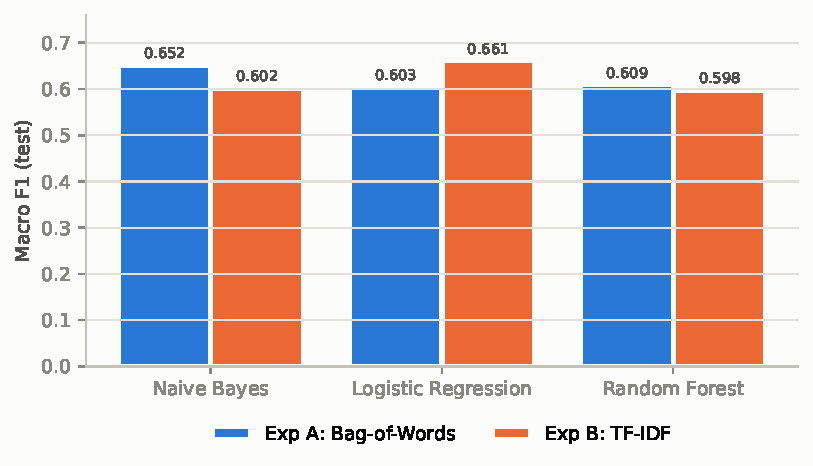
\includegraphics[width=1.0\linewidth]{fig1_macro_f1}
\caption{Test-set macro-F1 by model and feature representation.}
\label{fig:f1}
\end{figure}

Table~\ref{tab:metrics} and Fig.~\ref{fig:f1} summarise the six combinations. Logistic Regression with TF-IDF features achieved the highest macro-F1 (0.661) and accuracy (0.691), followed by Naive Bayes with BoW (0.652 and 0.680). The remaining four combinations fell in a narrow band of 0.598--0.609. The effect of term weighting depended on the model: TF-IDF raised Logistic Regression macro-F1 by 5.8 points over BoW, lowered Naive Bayes by 5.0 points and changed Random Forest by only $-1.1$ points. The Naive Bayes result is expected, since the multinomial model describes integer term counts and TF-IDF weighting departs from that assumption.

Cross-validated macro-F1 was within 2.2 points of the test value for every combination, so model selection did not overfit the particular split. Random Forest, however, fitted its training folds almost perfectly (training macro-F1 0.98) while generalising no better than the linear models, and its selected configuration lay on the upper edge of the grid (500 trees, depth 100) for both representations. Larger forests were not explored.

\subsection{Severe-Class Sensitivity}

\begin{figure}[!htbp]
\centering
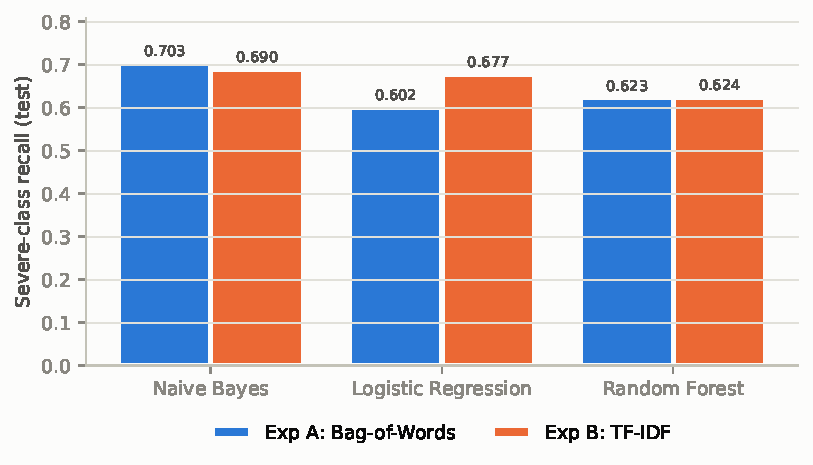
\includegraphics[width=1.0\linewidth]{fig1b_severe_recall}
\caption{Severe-class recall (sensitivity) on the test set.}
\label{fig:severe}
\end{figure}

Naive Bayes with BoW recalled the most Severe posts (0.703), ahead of Naive Bayes with TF-IDF (0.690) and Logistic Regression with TF-IDF (0.677); Random Forest reached 0.62 and Logistic Regression with BoW 0.60 (Fig.~\ref{fig:severe}). The best-balanced classifier and the most sensitive one therefore differ: Logistic Regression with TF-IDF misses about 2.5 more Severe posts per 100 than Naive Bayes with BoW. In every model, missed Severe posts went mainly to Mild (20--27\% of true Severe posts) rather than to Minimal (4--14\%) or Moderate (1--4\%).

\subsection{Error Analysis}

\begin{figure*}[!t]
\centering
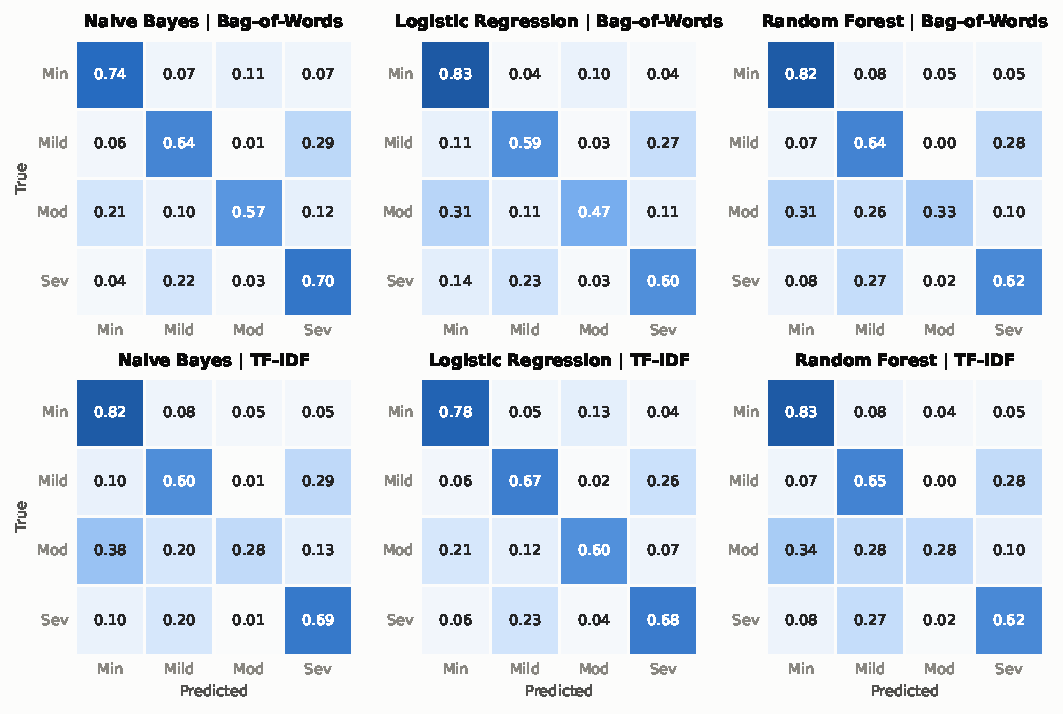
\includegraphics[width=\linewidth]{fig2_confusion_matrices}
\caption{Row-normalised confusion matrices. Cell $(i,j)$ is the share of true class $i$ predicted as class $j$ (Min = Minimal, Mod = Moderate, Sev = Severe).}
\label{fig:cm}
\end{figure*}

Fig.~\ref{fig:cm} shows that errors are not concentrated between adjacent severity levels. For every model, one of the two largest errors is Mild predicted as Severe (26--29\% of true Mild posts), and the reverse error (Severe predicted as Mild) is almost as large. Mild and Severe are two bands apart, so this pattern is more consistent with label noise or source-specific labelling conventions in the aggregated corpus than with genuinely borderline severity. Moderate is the hardest class (per-class F1 0.35--0.50): it is the smallest class after the audit (5.9\%), and 21--38\% of Moderate posts are predicted as Minimal, mirroring the \num{3028} texts that the audit found labelled both Minimal and Moderate.

\subsection{Interpretability}

\begin{figure}[!htbp]
\centering
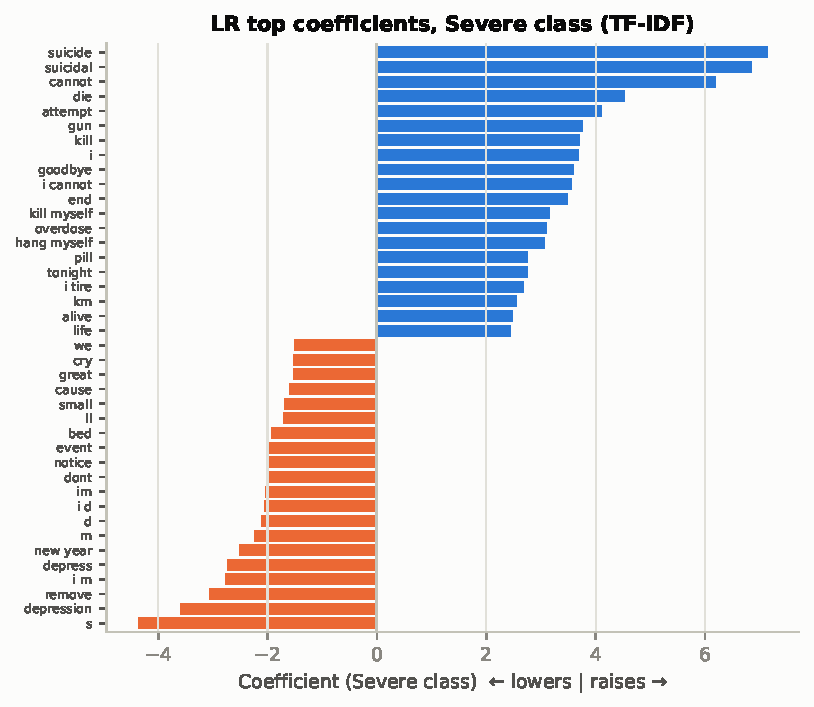
\includegraphics[width=1.0\linewidth]{fig3_lr_coefficients}
\caption{Largest positive and negative Logistic Regression coefficients for the Severe class (TF-IDF).}
\label{fig:lr}
\end{figure}

\begin{figure}[!htbp]
\centering
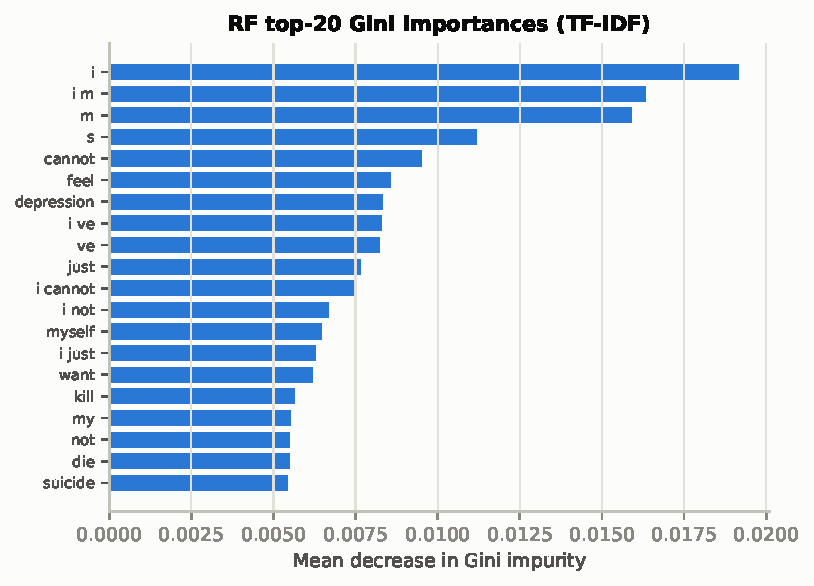
\includegraphics[width=1.0\linewidth]{fig4_rf_importances}
\caption{Top-20 Random Forest Gini importances (TF-IDF).}
\label{fig:rf}
\end{figure}

The L1 penalty assigned zero weight in all four classes to 39.0\% of the vocabulary in the TF-IDF Logistic Regression model. The largest positive Severe coefficients (Fig.~\ref{fig:lr}) are explicit suicidal-ideation and method terms---\textit{suicide}, \textit{suicidal}, \textit{die}, \textit{attempt}, \textit{kill}, \textit{gun}, \textit{goodbye}, \textit{kill myself}, \textit{overdose}, \textit{hang myself}, \textit{pill}, \textit{tonight}---together with the negation \textit{cannot}, the bigram \textit{i cannot} and the pronoun \textit{i}. Three of the ten strongest Severe markers (\textit{cannot}, \textit{i}, \textit{i cannot}) would have been deleted by the standard stop-word list, which supports retaining pronouns and negations. Random Forest importances (Fig.~\ref{fig:rf}) point the same way: \textit{i} is the single most important feature, and \textit{cannot}, \textit{myself}, \textit{i cannot}, \textit{i not}, \textit{my} and \textit{not} appear in the top~20 alongside \textit{kill}, \textit{die} and \textit{suicide}.

Among the negative Severe coefficients, \textit{depression} and \textit{depress} suggest that posts discussing depression as a topic were more often annotated as milder than posts expressing intent. Terms such as \textit{new year}, \textit{remove} and \textit{event} are more plausibly artefacts of individual source corpora than clinical markers. Tokens such as \textit{m}, \textit{s} and \textit{ve} are residue of the contractions \textit{I'm}, \textit{'s} and \textit{I've}, which our preprocessing did not expand (Section~\ref{sec:limits}).

\subsection{Effect of Duplicate Leakage}

\begin{table}[!htbp]
\centering
\caption{Macro-F1 on the audited vs.\ as-distributed corpus}
\label{tab:leak}
\begin{tabular}{llrrr}
\toprule
Features & Model & Audited & As distributed & $\Delta$ (points) \\
\midrule
BoW & Naive Bayes & 0.652 & 0.637 & -1.5 \\
TF-IDF & Naive Bayes & 0.602 & 0.639 & +3.7 \\
\bottomrule
\end{tabular}
\end{table}

Re-running Naive Bayes on the corpus as distributed (\num{41785} posts after removing empty texts) did not uniformly inflate scores (Table~\ref{tab:leak}): macro-F1 fell by 1.5 points with BoW and rose by 3.7 points with TF-IDF. Two effects act in opposite directions. Duplicates shared between the training and test sets let a model match memorised posts, which raises scores. The \num{3053} contradictorily labelled texts also enter the test set, where at most one of their labels can be predicted correctly, which lowers them. The net change therefore depends on the representation, and scores computed on the raw file are not comparable with scores on clean data in either direction. Logistic Regression and Random Forest were not re-run on the raw corpus because of their computational cost.

\subsection{Computational Efficiency}

\begin{table}[!htbp]
\centering
\caption{Training and inference cost of the selected configurations}
\label{tab:time}
\begin{tabular}{llrr}
\toprule
Features & Model & Train (s) & Predict (ms / 1k posts) \\
\midrule
BoW & Naive Bayes & 1.7 & 44.5 \\
BoW & Logistic Regression & 231.8 & 53.6 \\
BoW & Random Forest & 50.1 & 216.7 \\
TF-IDF & Naive Bayes & 1.8 & 45.5 \\
TF-IDF & Logistic Regression & 107.1 & 51.2 \\
TF-IDF & Random Forest & 77.3 & 256.7 \\
\bottomrule
\end{tabular}
\end{table}

Naive Bayes trained in under 2~s for either representation and completed its full grid search in under a minute (Table~\ref{tab:time}). Random Forest needed 50--77~s per fit with 500 trees, about 20 minutes per grid search on 4 cores, and was the slowest at inference (217--257~ms per \num{1000} posts including vectorisation, against 45--54~ms for the linear models). Logistic Regression was the most expensive to train (107~s with TF-IDF and 232~s with BoW per fit; 21 and 58 minutes per grid search) because SAGA converges slowly under an L1 penalty. Its selected configurations reached the 100-epoch limit before the $10^{-3}$ tolerance, so the reported coefficients are early-stopped solutions.

% ---------------------------------------------------------------------------
\section{Discussion}

\textbf{No single model dominates.} Logistic Regression with TF-IDF gives the best overall balance (macro-F1 0.661), but Naive Bayes with BoW is the most sensitive to Severe posts (recall 0.703), is within one macro-F1 point of the leader, and trains more than 50 times faster. For a first-stage screening tool, where missing a Severe case is the costliest error and models must be retrained cheaply as data changes, Naive Bayes with BoW is a strong default. Logistic Regression remains preferable where an auditable, sparse list of weighted markers is needed.

\textbf{The ceiling looks label-bound rather than model-bound.} Three model families with very different inductive biases---a generative linear model, a discriminative linear model and a non-linear ensemble---all landed between 0.60 and 0.66 macro-F1. Random Forest's near-perfect training fit did not translate into better test performance. Together with the large Mild$\leftrightarrow$Severe error and the Minimal/Moderate conflicts found in the audit, this points to inconsistent labels across the aggregated sources as the main limit, not insufficient model capacity. More complex models trained on the same labels are unlikely to remove it.

\textbf{The markers are clinically plausible but narrow.} The Severe class is driven largely by explicit suicidal-ideation vocabulary, which agrees with the clinical meaning of severe depression but also means the models may under-detect severe depression expressed without such words. The prominence of \textit{i}, \textit{cannot} and \textit{not} agrees with prior findings on self-focus and absolutist or negated language~\cite{rude2004language,almosaiwi2018absolute} and shows that preprocessing choices made before any model is trained can decide which of these signals survive.

\textbf{Audit before benchmarking.} The distributed file looks balanced only because Moderate posts were duplicated, and it contains texts with contradictory labels. Neither problem is visible from the class counts alone. Reporting the de-duplication procedure, and the corpus size after it, should be standard for severity datasets assembled from multiple sources.

% ---------------------------------------------------------------------------
\section{Limitations and Ethical Considerations}\label{sec:limits}

\textbf{Labels are not diagnoses.} Severity labels are text annotations aligned to BDI bands, not BDI scores collected from the people who wrote the posts. The models therefore learn to reproduce annotator judgements, and any deployment would be a screening aid that routes people to professional assessment, never a diagnostic instrument.

\textbf{Label noise.} The audit removed contradictions it could detect (identical text, different label). Near-duplicates and inconsistent labelling across \emph{different} texts cannot be detected this way and likely remain. The concentration of conflicts between Minimal and Moderate also suggests that one source corpus may be mis-mapped, which would affect the remaining Moderate posts as well. De-duplication was applied to raw text; after preprocessing, 33 test posts (0.6\%) became identical to training posts because they differed only in case, punctuation or URLs. Excluding them changed macro-F1 by at most 0.16 points and changed no ranking.

\textbf{Domain and language.} The corpus consists of English, largely social-media-style text. Performance on clinical notes, other platforms or other languages is untested.

\textbf{Lexical representation.} BoW and TF-IDF ignore word order beyond bigrams and cannot resolve sarcasm, quotation or third-person reports of another person's distress. The lexicon-augmented experiment (DSAS clinical keyword clusters) was not part of this study.

\textbf{Preprocessing and optimisation.} Only negative contractions were expanded, so \textit{I'm}, \textit{I've} and possessive \textit{'s} left fragments (\textit{m}, \textit{ve}, \textit{s}) in the vocabulary. Logistic Regression was early-stopped at 100 SAGA epochs, and the Random Forest optimum lay on the edge of its grid. Results come from one stratified split with a fixed seed; no significance tests between models were run, so differences of about one macro-F1 point should not be over-interpreted.

\textbf{Interpretability caveats.} Gini importance is biased towards high-frequency features~\cite{strobl2007bias}, and L1 selection among correlated features is unstable; both rankings indicate association, not causation.

\textbf{Privacy and harm.} Inferring mental-health status from text is sensitive. Any real use requires informed consent, data minimisation, human review of every Severe flag and a clear escalation path to crisis services.

% ---------------------------------------------------------------------------
\section{Conclusion and Future Work}

We benchmarked Naive Bayes, Logistic Regression and Random Forest with Bag-of-Words and TF-IDF features for four-level depression severity classification, after an audit that removed 29.9\% of the Depression Severity Levels Dataset as duplicate or contradictorily labelled. Logistic Regression with TF-IDF achieved the best macro-F1 (0.661), while Naive Bayes with BoW achieved the best Severe-class recall (0.703) at a fraction of the training cost. Severe predictions rest mainly on suicidal-ideation terms, first-person pronouns and negation, so stop-word lists should be adapted rather than applied as-is. All models plateaued near 0.66 macro-F1, which, together with the error structure, suggests that label consistency rather than model choice limits performance on this corpus.

Future work will (i)~add Experiment~C, concatenating scaled DSAS lexicon features with TF-IDF; (ii)~benchmark transformer models on the same audited split; (iii)~exploit the ordinal structure of severity with ordinal regression or cost-sensitive losses that penalise Severe-to-Minimal errors most; and (iv)~re-annotate the conflicting Minimal/Moderate posts with clinical experts.

\section*{Acknowledgment}
The authors thank the KUAS Ubiquitous Computing Lab for releasing the Depression Severity Levels Dataset openly.

\bibliographystyle{IEEEtran}
\bibliography{refs}

\end{document}
